\documentclass{bmvc2k}

%% Enter your paper number here for the review copy
%\bmvcreviewcopy{??}

%\usepackage[brazilian]{babel}
\usepackage[utf8]{inputenc}
\usepackage{bm}
\usepackage{amssymb}
\usepackage{amsmath}
\usepackage{tabularx}
\usepackage{siunitx}


\title{Projeto Demonstrativo 6: Reconhecimento de Faces}

% Enter the paper's authors in order
% \addauthor{Name}{email/homepage}{INSTITUTION_CODE}
\addauthor{Pedro Henrique Luz de Araujo}{pedrohluzaraujo@gmail.com}{1}
\addauthor{Raphael Soares Ramos}{raphael.soares.1996@gmail.com}{1}

% Enter the institutions
% \addinstitution{Name\\Address}
\addinstitution{
  Departamento de Ci\^encia da Comptuta\c{c}\~ao\\
  Universidade de Bras\'{\i}lia\\
  Campus Darcy Ribeiro, Asa Norte\\
  Bras\'{\i}lia-DF, CEP 70910-900, Brazil,  
}

\runninghead{Luz de Araujo, P.H.; Ramos, R.S.}{PD6 -- \today}

% Any macro definitions you would like to include
% These are not defined in the style file, because they don't begin
% with \bmva, so they might conflict with the user's own macros.
% The \bmvaOneDot macro adds a full stop unless there is one in the
% text already.
\def\eg{\emph{e.g}\bmvaOneDot}
\def\ie{\emph{i.e}\bmvaOneDot}
\def\Eg{\emph{E.g}\bmvaOneDot}
\def\etal{\emph{et al}\bmvaOneDot}
\newcommand{\norm}[1]{\left\lVert#1\right\rVert}
\newcommand\blfootnote[1]{%
  \begingroup
  \renewcommand\thefootnote{}\footnote{#1}%
  \addtocounter{footnote}{-1}%
  \endgroup
}


%-------------------------------------------------------------------------
% Document starts here
\begin{document}
\begin{NoHyper}
\maketitle
\end{NoHyper}

\begin{abstract}
O reconhecimento de faces tem como objetivo identificar faces de indivíduos específicos ou saber distinguir diferentes pessoas por meio de imagens das faces delas. No presente trabalho, desenvolvemos modelos treinados e avaliados em conjunto de dados de imagens de faces. O primeiro método implementado foi baseado em camadas completamente conectadas que têm como entrada vetores de imagens obtidos por rede convolucional profunda pré-treinada. Alcançamos resultados de acurácia no conjunto de validação superiores a 70\%. Já a segunda parte do trabalho visa a detectar e reconhecer faces a partir de \textit{face embeddings} obtidas do modelo OpenFace.
\footnote{Pedro contribuiu com a implementação, experimentos e testes da parte 1, além da escrita da introdução e partes da metodologia, resultados e conclusões referentes à parte 1. Raphael contribuiu com a implementação, experimentos e testes da parte 2, além da escrita das partes da metodologia, resultados e conclusões referentes à parte 2.}
\end{abstract}

%-------------------------------------------------------------------------
\section{Introdução}
\label{sec:intro}
%Histórico do reconhecimento de faces, falar do dataset%
O reconhecimento de faces é uma tarefa de visão computacional com variadas aplicações práticas, entre elas, sistemas de segurança, sistemas biométricos, interações humano e computador e indexação automática de imagens. Tal tarefa pode se referir a alguns subproblemas, como: dadas duas imagens de rostos, decidir se pertencem ao mesmo indivíduo; dada uma imagem de rosto, decidir se tal rosto pertence a um indivíduo específico; e dada uma imagem de rosto, verificar se o rosto pertence a algum indivíduo de um conjunto específico de pessoas~\cite{lfw}.

Em 1991, Turk e Pentland~\cite{eigenfaces} propuseram um método de reconhecimento de faces que se tornou extremamente popular. A técnica consistia em projetar as imagens de face em um espaço de características contendo as variações significantes entre as imagens. As características obtidas foram denominadas \textit{eigenfaces}, por serem os autovetores (\textit{eigenvectors}) do conjunto de faces. Uma vez obtidas as \textit{eigenfaces}, elas podem ser usadas para o reconhecimento de faces por meio da medição da distância entre imagens no espaço de características.

Mais recentemente, as técnicas estado-da-arte em reconhecimento de faces usam redes neurais convolucionais~\cite{siamese, triplet}. Além de obterem resultados muito melhores que outras técnicas de visão computacional, as redes neurais convolucionais têm a vantagem de dispensar a engenharia de características (\textit{feature engineering}).

No presente trabalho treinaremos e avaliaremos diferentes modelos treinados no \textit{dataset} de reconhecimento de faces \textit{Labeled Faces in the Wild}~\cite{lfw} (LFW). Ele contém 13233 imagens de 5749 indivíduos, entre os quais 1680 têm mais de uma imagem no \textit{dataset}. As imagens medem 250 por 250 pixeis e são resultantes de operações de re-escala e recorte em faces detectadas pelo detector Viola-Jones~\cite{viola}. O objetivo do modelo é, dadas duas imagens, classificá-las como pertencentes a mesma pessoa ou não.

%-------------------------------------------------------------------------
\section{Metodologia}
\label{sec:met}

%-------------------------------------------------------------------------
\subsection{Ferramentas}
Para realizar operações sobre matrizes e vetores, utilizamos a biblioteca de computação numérica em Python, NumPy. Usamos ainda, como linguagem, Python 3.5.2, e o gerenciador de bibliotecas Anaconda 3. Por fim, foram usadas as bibliotecas Keras~\cite{chollet2015keras} e Tensorflow~\cite{tensorflow2015-whitepaper} para o treinamento e construção de redes neurais. O treinamento foi realizado com o uso de uma placa de vídeo GeForce GTX 750 Ti.


%-------------------------------------------------------------------------
\subsection{Parte 1}
\subsubsection{O modelo}
%extraçao dicionario semelhança a siamese net%
A primeira parte do trabalho tem como objetivo analisar a viabilidade do uso de uma rede convolucional pré-treinada como extrator de características de imagens para reconhecimento facial. Foi usada para esse propósito uma rede Xception~\cite{xception} pré-treinada no ImageNet~\cite{imagenet}, base de dados com mais de 14 milhões de imagens.

A rede Xception é baseada em unidades de convoluções separáveis em profundidade (\textit{depthwise separable convolutions}), em que a convolução é separada em duas operações: uma convolução em profundidade, que é espacial e independente entre os canais de entrada; e uma por pontos, que projeta os canais obtidos da operação anterior em um novo espaço de canais.

Uma vez que inicializamos a rede com parâmetros aprendidos no ImageNet, a intuição é que ela possa servir como um extrator de características de imagens. Isto é, dada uma imagem, a rede deverá retornar um vetor capaz de descrevê-la, que servirá de entrada para um classificador. Para tanto, retiramos as ultimas camadas (totalmente conectadas) da Xception e substituímos por uma camada de \textit{average pooling} global em duas dimensões que retorna um vetor de 2048 dimensões.

Cada uma das imagens do LFW, com as faces já alinhadas pela técnica proposta por Huang~\cite{deepfunneling}, foi dada como entrada para a rede descrita, sendo salvos os vetores de saída em um dicionário. Dessa forma, não é necessário processar as imagens repetidas vezes durante o treino.

Para classificar as faces como pertencentes a mesma pessoa ou não, construímos um modelo inspirado no DeepFace~\cite{siamese}. Ele recebe como entrada um mapa de característica para cada um das duas imagens que serão comparadas, pré-calculados na etapa descrita acima. Em seguida ambos os vetores são combinados de alguma forma~\footnote{Mais sobre isso na seção de experimentos.} e passam por uma camada completamente conectada e uma camada de Dropout~\cite{dropout} seguida por uma unidade com ativação sigmóide que gera a classificação.


\subsubsection{Experimentos}
%dataset com faces já alinhadas, hiperparametros e callables%
Realizamos experimentos variando três hiper-parâmetros e avaliando os resultados no conjunto de validação do \textit{dataset}. A separação entre treino e validação já foi feita pelos criadores do dataset e consiste em 2200 pares de imagem para treinamento e 1000 pares para validação. Em cada um dos conjuntos, metade dos pares corresponde a faces do mesmo indivíduo (exemplos positivos) e a outra metade a faces de indivíduos diferentes (exemplos negativos).

Variamos conjuntamente o número de unidades da camada completamente conectada (128, 512 ou 1024) e o valor de probabilidade de Dropout (0.2, 0.5, 0.8). Uma vez obtidos os melhores valores para esses hiperparâmetros, experimentamos diferentes maneiras de combinar os vetores de características das duas imagens de entrada (soma, concatenação, subtração, produto interno e produto elemento a elemento). Dessa forma, ao todo foram treinados 14 modelos diferentes.

Como otimizador usamos \textit{rmsprop}~\cite{rmsprop} para minimizar a função de entropia cruzada binária. Sejam $p$ a previsão da rede e $y$ o rótulo que se deseja prever, a função de entropia cruzada binária é

\begin{equation}
    \textit{cross-entropy} = -{(y\log(p) + (1 - y)\log(1 - p))}\,.
\end{equation}
O tamanho de \textit{batch} usado foi 128 e o modelo foi treinado por 60 épocas, sendo que o salvamos apenas quando houvesse melhora na acurácia do conjunto de validação.



%-------------------------------------------------------------------------
\subsection{Parte 2}
\label{pt2}
\subsubsection{O modelo}
Na segunda do parte do trabalho foi realizado: detecção de faces; cálculo das \textit{face embeddings} para quantificar a face; treino de uma \textit{Support Vector Machine}~\cite{hearst1998support} (SVM) nas embeddings; reconhecimento de faces em imagens e vídeos. Para construir esse pipeline foi usado modelos de redes neurais profundas em dois pontos chaves: detecção de faces e extração dos vetores de 128 características (\textit{embeddings}) que quantificam cada face na imagem. Uma \textit{embedding} é representado por $f(x) \in \mathbb{R}^d$. Ela incorpora uma imagem $x$ em um espaço euclidiano de $d$-dimensões.

O modelo responsável por quantificar cada face na imagem pertence ao projeto \textit{OpenFace}~\cite{amos2016openface}, que é uma implementação em Python e Torch~\cite{torch} de reconhecimento de faces com redes neurais profundas. Esta implementação veio da publicação do paper ~\cite{triplet}.

A rede do modelo \textit{OpenFace} (\textit{FaceNet}) é treinada para calcular as face embeddings de uma forma diferente. Cada \textit{batch} dos dados inclui três imagens: a âncora (imagem atual), a imagem positiva e a imagem negativa. A âncora e a imagem positiva pertencem à mesma pessoa/face, enquanto as imagens negativas não. A rede neural computa as embeddings para cada face e então atualiza os pesos da rede usando a função \textit{triplet loss} como parâmetro, conforme mostra a figura \ref{fig:triplet}. É computada uma função $f(x)$, de uma imagem $x$ em um espaço de características $\mathbb{R}^d$ de modo que a distância euclidiana entre todas as faces, independente das condições da imagem, de mesma identidade é pequena, enquanto a distância entre pares de imagens de diferentes identidades é grande. A rede consiste de uma \textit{batch input layer} e uma rede neural convolucional profunda seguida por normalização $L_2$, que resulta na face embedding. Esse processo é seguido pela \textit{triplet loss} durante o treinamento. 	

\begin{figure}[htb]
\begin{center}
\begin{tabular}{c}
	\bmvaHangBox{\fbox{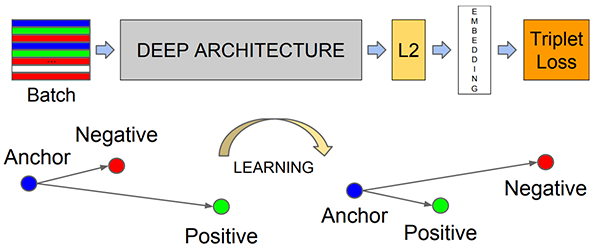
\includegraphics[width=5cm]{figs/triplet_loss.png}}}
\end{tabular}
\end{center}
\caption{Estrutura do modelo utilizado.}
\label{fig:triplet}
\end{figure}

\subsubsection{Experimentos}
Foram feitos experimentos no dataset LFW sem alinhamento e em um dataset gerado a partir dos alunos da turma. Em ambos os datasets é realizada a detecção e reconhecimento de faces. Foi selecionado um subconjunto do LFW para treino e um para teste. O mesmo foi feito com dataset gerado.

Primeiro é aplicado um detector de faces da OpenCV~\cite{opencvmanual} para localizar e detectar faces nas imagens de entrada. Então, assumindo que cada imagem possui apenas um rosto, é proucrada uma região de interesse com maior probabilidade de conter um rosto e é verificado se essa probabilidade é maior do que uma constante estabelecida. Depois, esta região de interesse é passada pela rede convolucional profunda para gerar um vetor que descreve a face (\textit{embedding}). Por fim, o modelo \textit{SVM} é treinado para reconhecer novas faces.

%-------------------------------------------------------------------------
\section{Resultados}
\label{sec:res}

%-------------------------------------------------------------------------
\subsection{Parte 1}
\label{res:req1}
%tabela com resultados hiper e merge e imagem com resultados velocidade%
A figura~\ref{fig:curve} exibe a acurácia de treino e validação para diferentes valores dos hiperparâmetros dropout e número de unidades ao longo do treinamento. A figura~\ref{fig:merge} é análoga, mas corresponde aos modelos treinados com diferentes métodos de combinação de característica das imagens.

\begin{figure}[htb]
\centering
    \centering
    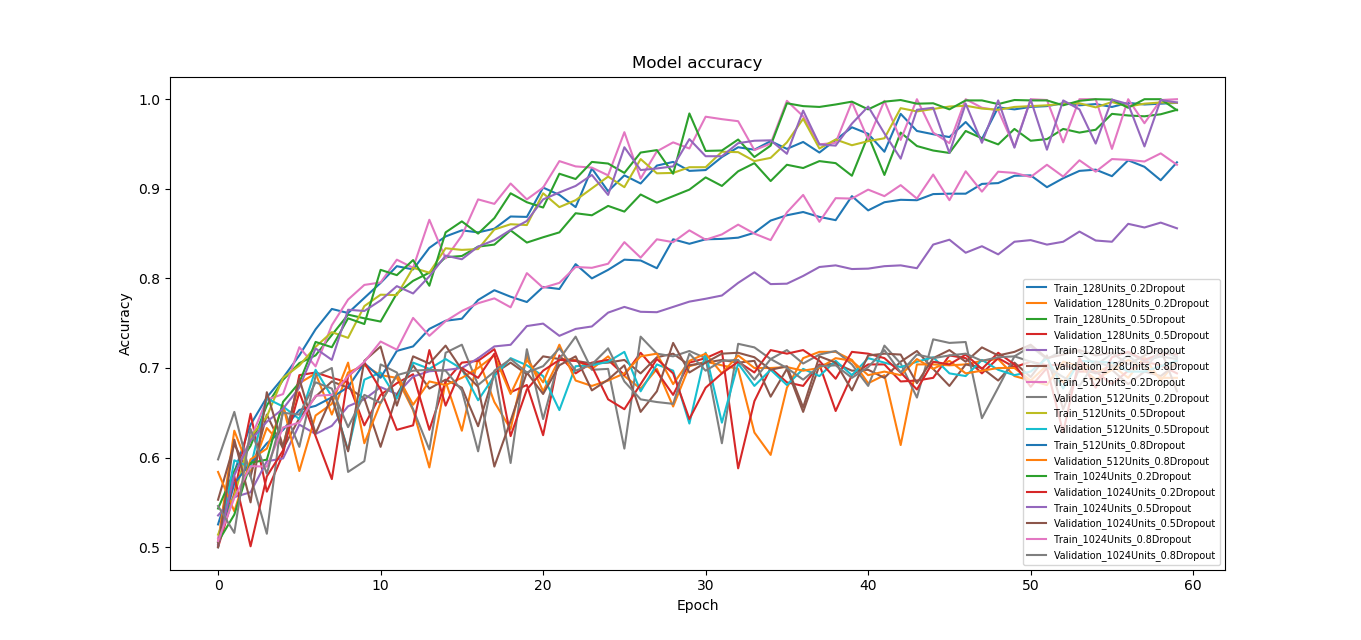
\includegraphics[width=\textwidth]{figs/curve.png}
    \caption{Acurácia no treino e na validação ao longo do treinamento para diferentes valores de dropout e número de unidades.}
    \label{fig:curve}
\end{figure}

\begin{figure}[htb]
    \centering
    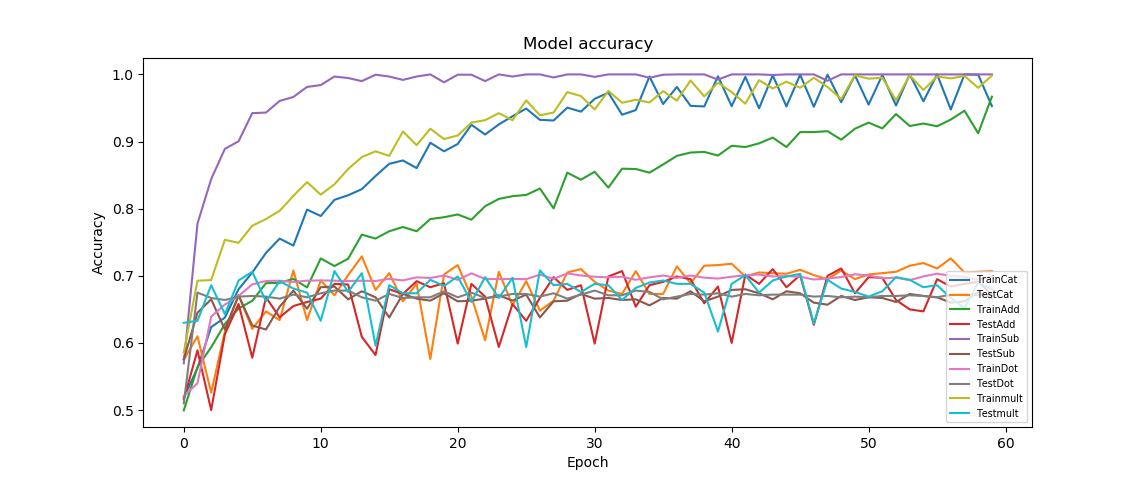
\includegraphics[width=\textwidth]{figs/curve_merge.png}
    \caption{Acurácia no treino e na validação ao longo do treinamento para diferentes combinações de características de imagens.}
    \label{fig:merge}
\end{figure}

A Tabela~\ref{tab:dropunit} exibe os valores de acurácia na validação para cada um dos modelos treinados variando número de unidades e dropout. A Tabela~\ref{tab:merge} exibe a mesma métrica para modelos treinados com 512 unidades e 20\% de dropout e diferentes métodos de combinação.

\begin{table}[htb]
    \small
    \centering
    \begin{tabular}{|l|c|}
        \hline
        Modelo & Acurácia \\
        \hline
        Units\_128\_Drop\_0.2 & 0.718 \\
        Units\_128\_Drop\_0.5 & 0.721 \\
        Units\_128\_Drop\_0.8 & 0.719 \\
        Units\_512\_Drop\_0.2 & \textbf{0.735} \\
        Units\_512\_Drop\_0.5 & 0.718 \\
        Units\_512\_Drop\_0.8 & 0.726 \\
        Units\_1024\_Drop\_0.2 & 0.72 \\
        Units\_1024\_Drop\_0.5 & 0.728 \\
        Units\_1024\_Drop\_0.8 & 0.722 \\
        \hline
    \end{tabular}
    \caption{Resultados no conjunto de validação para o primeiro cenário de experimento de hiper-parâmetro.}
    \label{tab:dropunit}
\end{table}

\begin{table}[htb]
    \small
    \centering
    \begin{tabular}{|l|c|}
        \hline
        Modelo & Acurácia \\
        \hline
        concat & \textbf{0.729} \\
        add & 0.711 \\
        subtract & 0.684 \\
        dotProduct & 0.678 \\
        multiply & 0.708 \\
        \hline

    \end{tabular}
    \caption{Resultados no conjunto de validação para o segundo cenário de experimento de hiper-parâmetro.}
    \label{tab:merge}
\end{table}

O treinamento do modelo mostrou-se extremamente rápido, uma vez que as características das imagens fora previamente computada, levando menos de um minuto para concluir 60 épocas.

%-------------------------------------------------------------------------
\subsection{Parte 2}
Nas figuras \ref{fig:angelina}, \ref{fig:Robert} e \ref{fig:laura} é testado o modelo construído de detecção e reconhecimentos de faces com imagens não vistas anteriormente pelo modelo.

\begin{figure}[htb]
\begin{center}
\begin{tabular}{cc}
	\bmvaHangBox{\fbox{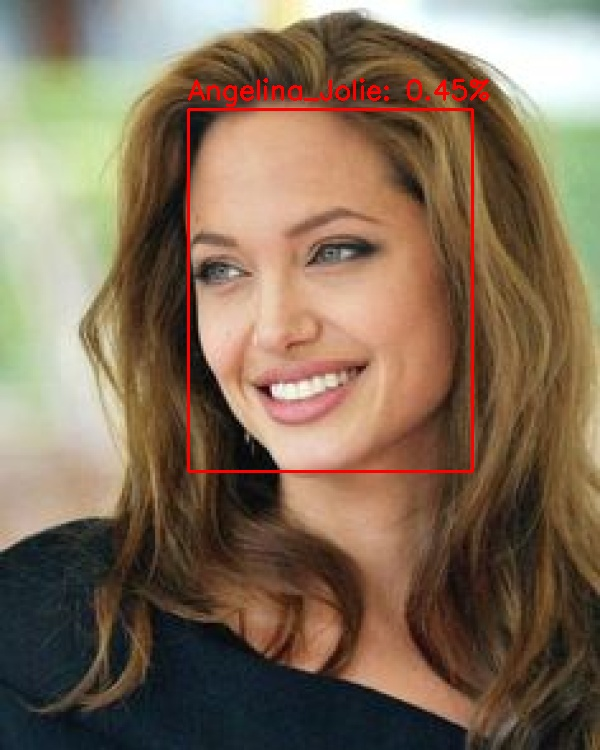
\includegraphics[width=30mm]{figs/Angelina_Jolie_2.jpg}}} &
	\bmvaHangBox{\fbox{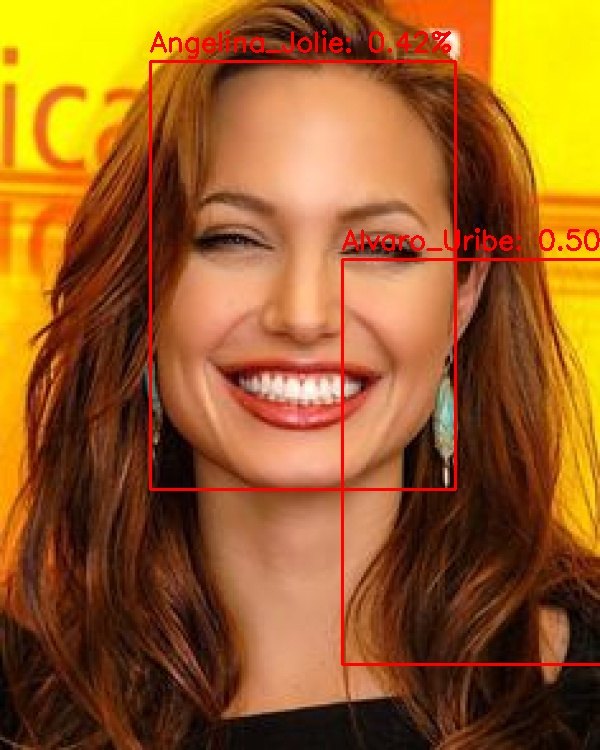
\includegraphics[width=30mm]{figs/Angelina_Jolie_3.jpg}}} \\
\end{tabular}
\end{center}
\caption{Fotos da Angelina Jolie testadas no pipeline construído de detecção e reconhecimento de faces.}
\label{fig:angelina}
\end{figure}

\begin{figure}[htb]
\begin{center}
\begin{tabular}{ccc}
	\bmvaHangBox{\fbox{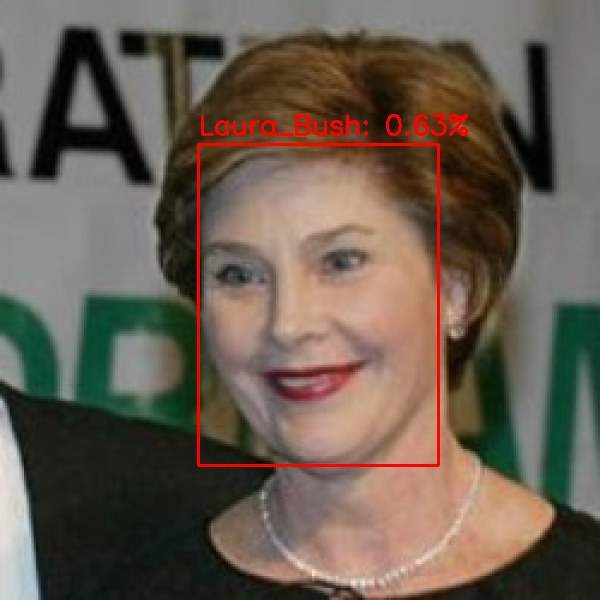
\includegraphics[width=30mm]{figs/Laura_Bush_0036.jpg}}} &
  	\bmvaHangBox{\fbox{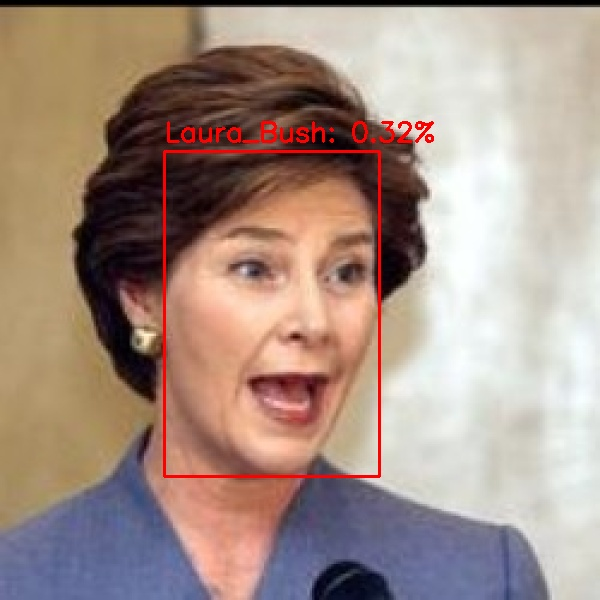
\includegraphics[width=30mm]{figs/Laura_Bush_0037.jpg}}} &
  	\bmvaHangBox{\fbox{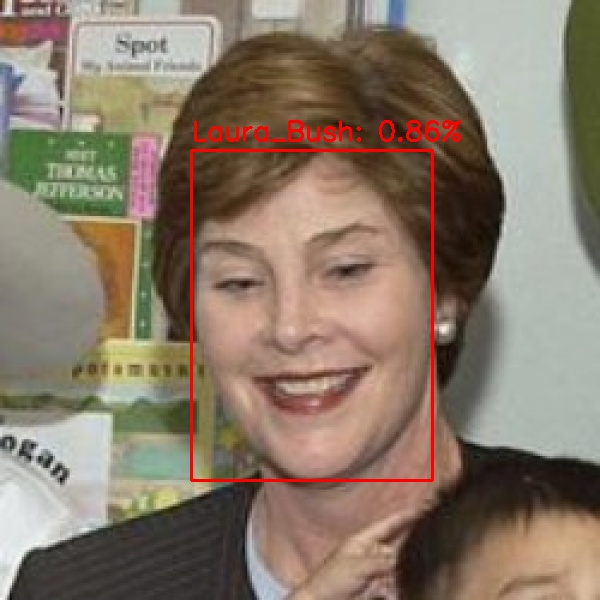
\includegraphics[width=30mm]{figs/Laura_Bush_0038.jpg}}} \\
\end{tabular}
\end{center}
\caption{Fotos da Laura Bush testadas no pipeline construído de detecção e reconhecimento de faces.}
\label{fig:laura}
\end{figure}

\begin{figure}[htb]
\begin{center}
\begin{tabular}{cc}
	\bmvaHangBox{\fbox{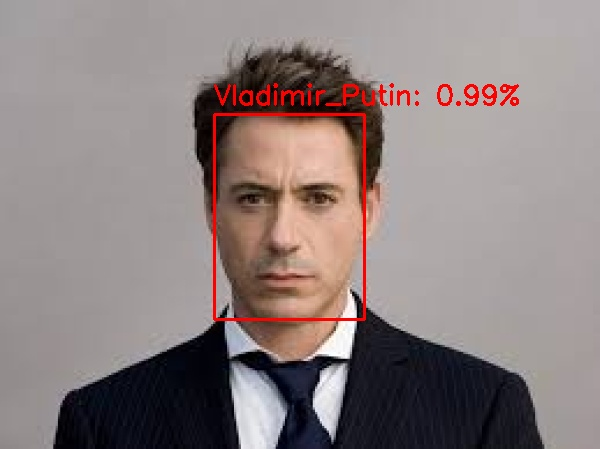
\includegraphics[width=30mm]{figs/Robert_Downey_Jr_2.jpg}}} &
	\bmvaHangBox{\fbox{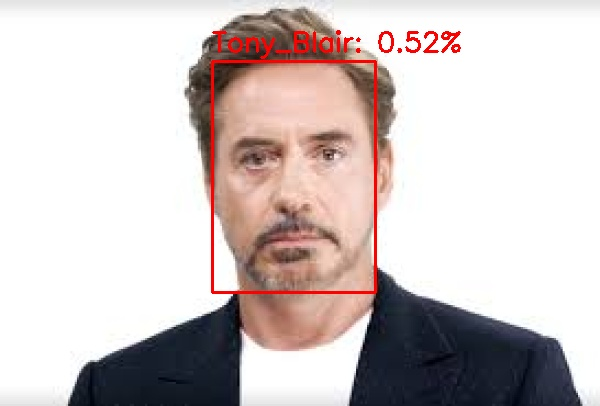
\includegraphics[width=30mm]{figs/Robert_Downey_Jr_3.jpg}}} \\
\end{tabular}
\end{center}
\caption{Fotos do Robert Downey Jr testadas no pipeline construído de detecção e reconhecimento de faces. A classificação dada aqui foi errada.}
\label{fig:Robert}
\end{figure}	

%-------------------------------------------------------------------------
\section{Discussão e Conclusões}
\label{sec:conc}

%Overfitting, velocidade, testar com mais dados, pesos pretreinados no dominio correto falar dos diferentes merge, usar triplet loss%
O modelo apresentado na Parte 1 conseguiu superar a \textit{baseline} do conjunto de validação, alcançando 73,5\% de acurácia, contra os 50\% de \textit{baseline}. O método de combinação das entradas que obteve melhor resultado foi a concatenação. Isso pode ser explicado pelo fato de a concatenação permitir que o modelo aprenda operações arbitrárias sobre as características das imagens em vez de se restringir a uma operação escolhida pelo usuário.

Por outro lado, nota-se das figuras~\ref{fig:curve} e~\ref{fig:merge} que ocorre \textit{overfitting}. Isso porque há grande distância entre a acurácia na validação e no treino, que chega por vezes a 100\%. Isso sugere que o modelo está aprendendo a classificar imagens não por meio do que realmente importa, isto é, as propriedades das faces, mas sim por outros elementos da imagem (iluminação, expressão facial, \textit{background}). Esse problema de \textit{overfitting} também foi encontrado por Taigman et al.~\cite{siamese} por causa do reduzido tamanho do conjunto de treino.

Assim, seria interessante avaliar a performance do modelo em \textit{datasets} maiores, a fim de reduzir o \textit{overfitting}. Outra possível via de melhoria seria o uso de pesos do extrator pré-treinados em um conjunto de imagens do domínio de reconhecimento facial. Afinal, parte do erro de generalização do modelo pode se dar ao fato de o extrator ter ``aprendido'' a reconhecer objetos e não rostos. Por fim, uma maneira de aumentar o tamanho do \textit{dataset} seria por meio da função custo \textit{triplet loss}~\cite{triplet}. Dessa forma, o treinamento não ficaria restrito aos pares pré-selecionados de faces.

Dito isso, a técnica apresenta como vantagem a grande rapidez de treinamento, a simplicidade do modelo e desnecessidade de gerar características manualmente. Mostra-se necessário fazer as melhorias elencadas acima para avaliar a viabilidade do modelo para usos práticos.

O modelo apresentado na parte 2, por outro lado, mostrou-se muito bom para a detecção de faces, embora não tenha uma performance tão boa quanto ao reconhecimento de pessoa. Isso não é surpreendente, visto que há grande número de classes, muitas delas com poucos exemplos de treinamento. Seria interessante em um trabalho futuro avaliar o modelo no mesmo \textit{dataset} usado na parte 1 a fim de comparar os resultados.


\bibliography{refs}
\end{document}
